\chapter{Database Scanning}

\section{Overview}

Database scanning is the mechanism for deciding when to process a record.
Five types of scanning are possible:

\begin{itemize}
\item \index{Periodic - Scan Type}Periodic: A record can be processed periodically.
A number of time intervals are supported.

\item \index{Event - Scan Type}Event: Event scanning is based on the posting of an event by another component of the software via a call to the routine \verb|post_event|.

\item \index{I/O Event - Scan Type}I/O Event: The original meaning of this scan type is a request for record processing as a result of a hardware interrupt.
The mechanism supports hardware interrupts as well as software generated events.

\item \index{Passive - Scan Type}Passive: Passive records are processed only via requests to \verb|dbScanPassive|.
This happens when database links (Forward, Input, or Output), which have been declared ``Process Passive" are accessed during record processing.
It can also happen as a result of \verb|dbPutField| being called (which normally results from a Channel Access put request).

\item \index{Scan Once - Scan Type}Scan Once: In order to provide for caching puts, the scanning system provides a routine \verb|scanOnce| which arranges for a record to be processed one time.

\end{itemize}

This chapter explains database scanning in increasing order of detail.
It first explains database fields involved with scanning.
It next discusses the interface to the scanning system.
The last section gives a brief overview of how the scanners are implemented.

\section{Scan Related Database Fields}

\index{Scan Related Database Fields}
The following fields are normally defined via DCT.
It should be noted, however, that it is quite permissible to change any of the scan related fields of a record dynamically.
For example, a display manager screen could tie a menu control to the \verb|SCAN| field of a record and allow the operator to dynamically change the scan mechanism.

\subsection{SCAN}

\index{SCAN - Scan Related Field}
This field, which specifies the scan mechanism, has an associated menu of the following form:

\begin{description}
\item \index{Passive}Passive: Passively scanned.

\item \index{Event}Event: Event Scanned. The field \verb|EVNT| specifies event number.

\item \index{I/O Event scanned}I/O Intr: I/O Event scanned.

\item 10 Second: Periodically scanned every 10 seconds

\item ...

\item .1 Second: Periodically scanned every .1 seconds

\end{description}

\subsection{PHAS}

\index{PHAS - Scan Related Field}
This field determines processing order for records that are in the same scan set.
For example all records periodically scanned at a 2 second rate are in the same scan set.
All Event scanned records with the same \verb|EVNT| are in the same scan set, etc.
For records in the same scan set, all records with \verb|PHAS|=0 are processed before records with \verb|PHAS|=1, which are processed before all records with \verb|PHAS|=2, etc.

In general it is not a good idea to rely on \verb|PHAS| to enforce processing order.
It is better to use database links.

\subsection{EVNT - Event Number}

\index{EVNT - Scan Related Field}
This field only has meaning when \verb|SCAN| is set to \verb|Event| scanning, in which case it specifies the event number.
In order for a record to be event scanned, \verb|EVNT| must be in the range 0,...255.
It should also be noted that some EPICS software components will not request event scanning for event 0.
One example is the \verb|eventRecord| record support module.
Thus the application developer will normally want to define events in the range 1,...,255.

\subsection{PRIO - Scheduling Priority }

\index{PRIO - Scan Related Field}
This field can be used by any software component that needs to specify scheduling priority, e.g. the event and I/O event scan facility uses this field.

\section{Scan Related Software Components}

\subsection{menuScan.dbd}

\index{menuScan.dbd}
This file contains definitions for a menu related to field \verb|SCAN|.
The definitions are of the form:

\begin{verbatim}
menu(menuScan) {
    choice(menuScanPassive,"Passive")
    choice(menuScanEvent,"Event")
    choice(menuScanI_O_Intr,"I/O Intr")
    choice(menuScan10_second,"10 second")
    choice(menuScan5_second,"5 second")
    choice(menuScan2_second,"2 second")
    choice(menuScan1_second,"1 second")
    choice(menuScan_5_second,".5 second")
    choice(menuScan_2_second,".2 second")
    choice(menuScan_1_second,".1 second")
}
\end{verbatim}

The first three choices must appear in the order and location shown.
The remaining definitions are for the periodic scan rates, which must appear in the order slowest to fastest (the order directly controls the thread priority assigned to the particular scan rate, and faster scan rates should be assigned higher thread priorities).
At IOC initialization, the menu choice strings are read at scan initialization.
The number of periodic scan rates and the period of each rate is determined from the menu choice strings.
Thus periodic scan rates can be changed by changing \verb|menuScan.dbd| and loading this version via \verb|dbLoadDatabase|.
The only requirement is that each periodic choice string must begin with a numeric value specified in units of seconds.

\subsection{dbScan.h}

\index{dbScan.h}
All software components that interact with the scanning system must include this file.

The most important definitions in this file are:

\begin{verbatim}
#define SCAN_PASSIVE       menuScanPassive
#define SCAN_EVENT         menuScanEvent
#define SCAN_IO_EVENT      menuScanI_O_Intr
#define SCAN_1ST_PERIODIC  (menuScanI_O_Intr + 1)

/*definitions for I/O Interrupt Scanning */
typedef struct io_scan_list *IOSCANPVT;
typedef void (*io_scan_complete)(void *, IOSCANPVT, int);

long scanInit(void);
void scanRun(void);
void scanPause(void);

void post_event(int event);
void scanAdd(struct dbCommon *);
void scanDelete(struct dbCommon *);
double scanPeriod(int scan);
void scanOnce(struct dbCommon *precord);
int scanOnceSetQueueSize(int size);

int scanppl(void);    /* print periodic lists*/
int scanpel(void);    /* print event lists*/
int scanpiol(void);   /* print io_event list*/

void scanIoInit(IOSCANPVT *);
unsigned int scanIoRequest(IOSCANPVT);
void scanIoSetComplete(IOSCANPVT, io_scan_complete, void*);
\end{verbatim}

\index{SCAN\_1ST\_PERIODIC}The first set of definitions defines the various scan types.
The next definition \verb|IOSCANPVT| is used when interfacing with the I/O interrupt scanner.
The remaining definitions define the public scan access routines.
These are described in the following subsections.

\subsection{Initializing And Controlling Database Scaning}

\begin{verbatim}
scanInit(void);
\end{verbatim}

\index{scanInit}The routine \verb|scanInit| is called by \verb|iocInit|.
It initializes the scanning system.

\begin{verbatim}
scanRun(void);
scanPause(void);
\end{verbatim}

\index{scanRun}
\index{scanPause}
These routines start and stop all the scan tasks respectively.
They are used by the \verb|iocInit|, \verb|iocRun| and \verb|iocPause| commands.

\subsection{Adding And Deleting Records From Scan List}

The following routines are called each time a record is added or deleted from a scan list.

\begin{verbatim}
scanAdd(struct dbCommon *);
scanDelete(struct dbCommon *);
\end{verbatim}

\index{scanAdd}
\index{scanDelete}
These routines are called by \verb|scanInit| at IOC initialization time in order to enter all records created via DCT into the correct scan list.
The routine \verb|dbPut| calls \verb|scanDelete| and \verb|scanAdd| each time a scan related field is changed (each scan related field is declared to be \verb|SPC_SCAN| in \verb|dbCommon.dbd|).
\verb|scanDelete| is called before the field is modified and \verb|scanAdd| after the field is modified.

\subsection{Obtaining the scan period from the SCAN field}

\begin{verbatim}
double scanPeriod(int scan);
\end{verbatim}

\index{scanPeriod}The argument is an offset into the set of enum choices for menuScan.h.
Most users will just use the SCAN field of a database record.
It returns the scan period in seconds.
The result will be 0.0 if scan doesn't refer to a periodic rate.

\subsection{Declaring Database Event}

Whenever any software component wants to declare a database event, it just calls:

\begin{verbatim}
post_event(event)
\end{verbatim}

\index{post\_event}This can be called by virtually any IOC software component.
For example sequence programs can call it.
The record support module for \verb|eventRecord| calls it.

\subsection{Interfacing to I/O Event Scanning}

\index{I/O Event Scanning}

Interfacing to the I/O event scanner is done via some combination of device and driver support.

\begin{enumerate}
\item Include \verb|<dbScan.h>|

\item For each separate I/O event source the following must be done:

\begin{enumerate}

\item Declare an \verb|IOSCANPVT| variable, e.g.

\begin{verbatim}
static IOSCANPVT ioscanpvt;
\end{verbatim}

\item Call \verb|scanIoInit|, e.g.

\begin{verbatim}
scanIoInit(&ioscanpvt);
\end{verbatim}
\end{enumerate}

\item Provide the device support \verb|get_ioint_info| routine.
This routine has the format:

\begin{verbatim}
long get_ioint_info(
    int cmd,
    struct dbCommon *precord,
    IOSCANPVT *ppvt);
\end{verbatim}

This routine is called each time the record pointed to by \verb|precord| is added or deleted from an I/O event scan list.
\verb|cmd| has the value (0,1) if the record is being (added to, deleted from) an I/O event list.
This routine must give a value to \verb|*ppvt|.

\item Whenever an I/O event is detected call \verb|scanIoRequest|, e.g.

\begin{verbatim}
scanIoRequest(ioscanpvt);
\end{verbatim}

This routine can be called from interrupt level.
The request is queued and will be handled by one of the standard callback threads.
There are three sets of callback threads fed from three queues, one for each priority level (see \ref{sec:callbackThreads}); the \verb|PRIO| field of a record determines which queue will be used for processing this record after \verb|scanIoRequest()| has been called.

\verb|scanIoRequest()| now returns a bit pattern indicating which of the three queues the request was sent to.
A return value of zero means no records are currently configured to use this interrupt source for I/O Interrupt scanning.

Device or driver support that needs to implement flow control can set up a completion callback by calling \verb|scanIoSetComplete|, e.g.

\begin{verbatim}
static void myCallback(void *arg, IOSCANPVT pvt, int prio)
{
    [...]
}

scanIoSetComplete(ioscanpvt, myCallback, (void *)arg);
\end{verbatim}

The completion callback will be called from one of the callback threads, once per priority used (bits set in the return value of \verb|scanIoRequest|), after the list of records with that priority level has been processed. Note that for records with asynchronous device support, record processing might not have completed when the callback is issued.
\end{enumerate}

The following code fragment shows an event record device support module that supports I/O event scanning: 

\begin{verbatim}
#include  <vxWorks.h>
#include  <types.h>
#include  <stdioLib.h>
#include  <intLib.h>
#include  <dbDefs.h>
#include  <dbAccess.h>
#include  <dbScan.h>
#include  <recSup.h>
#include  <devSup.h>
#include  <eventRecord.h>
/* Create the dset for devEventXXX */
long init();
long get_ioint_info();
struct {
    long  number;
    DEVSUPFUN  report;
    DEVSUPFUN  init;
    DEVSUPFUN  init_record;
    DEVSUPFUN  get_ioint_info;
    DEVSUPFUN  read_event;
}devEventTestIoEvent={
    5,
    NULL,
    init,
    NULL,
    get_ioint_info,
    NULL};
static IOSCANPVT ioscanpvt;
static void int_service(IOSCANPVT ioscanpvt)
{
    scanIoRequest(ioscanpvt);
}

static long init()
{
    scanIoInit(&ioscanpvt);
    intConnect(<vector>,(FUNCPTR)int_service,ioscanpvt);
    return(0);
}
static long get_ioint_info(
int   cmd,
struct eventRecord   *pr,
IOSCANPVT   *ppvt)
{
    *ppvt = ioscanpvt;
    return(0);
}
\end{verbatim}

\index{get\_ioint\_info}\section{Implementation Overview}

The code for the entire scanning system resides in \verb|dbScan.c|, i.e. periodic, event, and I/O event.
This section gives an overview of how the code in \verb|dbScan.c| is organized.
The listing of \verb|dbScan.c| must be studied for a complete understanding of how the scanning system works.

\subsection{Definitions And Routines Common To All Scan Types}

Everything is built around two basic structures:

\begin{verbatim}
typedef struct scan_list {
    epicsMutexId lock;
    ELLLIST      list;
    short        modified;
};

typedef struct scan_element{
    ELLNODE         node;
    scan_list       *pscan_list;
    struct dbCommon *precord;
}
\end{verbatim}

Later we will see how \verb|scan_list|s are determined.
For now just realize that \verb|scan_list.list| is the head of a list of records that belong to the same scan set (for example, all records that are periodically scanned at a 1 second rate are in the same scan set).
The node field in \verb|scan_element| contain the list links.
The normal libCom \verb|ellLib| routines are used to access the list.
Each record that appears in some scan list has an associated \verb|scan_element|.
The \verb|SPVT| field which appears in \verb|dbCommon| holds the address of the associated \verb|scan_element|.

The \verb|lock|, \verb|modified|, and \verb|pscan_list| fields allow \verb|scan_elements|, i.e. records, to be dynamically removed and added to scan lists.
If \verb|scanList|, the routine which actually processes a scan list, is studied it can be seen that these fields allow the list to be scanned very efficiently if no modifications are made to the list while it is being scanned.
This is, of course, the normal case.

The \verb|dbScan.c| module contains several private routines. The following access a single scan set: 

\begin{itemize}
\item printList: Prints the names of all records in a scan set.

\item scanList: This routine is the heart of the scanning system.
For each record in a scan set it does the following:

\begin{verbatim}
dbScanLock(precord);
dbProcess(precord);
dbScanUnlock(precord);
\end{verbatim}

It also has code to recognize when a scan list is modified while the scan set is being processed.

\item addToList: This routine adds a new element to a scan list.

\item deleteFromList: This routine deletes an element from a scan list.

\end{itemize}

\subsection{Event Scanning}

\index{Event Scanning}
Event scanning is built around the following definitions:

\begin{verbatim}
#define MAX_EVENTS 256
typedef struct event_scan_list {
    CALLBACK        callback;
    scan_list       scan_list;
} event_scan_list;
static event_scan_list
*pevent_list[NUM_CALLBACK_PRIORITIES][MAX_EVENTS];
\end{verbatim}

\verb|pevent_list| is a 2d array of pointers to \verb|scan_lists|.
Note that the array allows for 256 events, i.e. one for each possible event number.
In other words, each event number and priority has its own scan list.
No \verb|scan_list| is actually created until the first request to add an element for that event number.
The event scan lists have the memory layout illustrated below:

\begin{center}
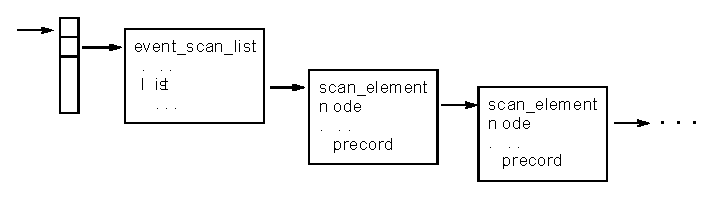
\includegraphics{scanning_12}
\end{center}

\subsubsection{post\_event} \index{post\_event}

\begin{verbatim}
post_event(int event)
\end{verbatim}

\index{post\_event}This routine is called to request event scanning.
It can be called from interrupt level.
It looks at each \verb|event_scan_list| referenced by \verb|pevent_list[*][event]| (one for each callback priority) and if any elements are present in the \verb|scan_list| a \verb|callbackRequest| is issued.
The appropriate callback task calls routine \verb|eventCallback|, which just calls \verb|scanList|. 

\subsection{I/O Event Scanning}

\index{I/O Event Scanning}
I/O event scanning is built around the following definitions:

\begin{verbatim}
typedef struct io_scan_list {
    CALLBACK            callback;
    scan_list           scan_list;
    struct io_scan_list *next;
}
static io_scan_list *iosl_head[NUM_CALLBACK_PRIORITIES] = {
    NULL,NULL,NULL};
\end{verbatim}

The array \verb|iosl_head| and the field \verb|next| are only kept so that \verb|scanpiol| can be implemented and will not be discussed further.
I/O event scanning uses the general purpose callback tasks to perform record processing, i.e. no task is spawned for I/O event.
The callback field of \verb|io_scan_list| is used to communicate with the callback tasks.

The following routines implement I/O event scanning:

\subsubsection{scanIoInit}

\begin{verbatim}
scanIoInit (IOSCANPVT  *ppioscanpvt)
\end{verbatim}

\index{scanIoInit}This routine is called by device or driver support.
It is called once for each interrupt source.
\verb|scanIoInit| allocates and initializes an array of \verb|io_scan_list| structures; one for each callback priority and puts the address in \verb|pioscanpvt|.
Three callback priorities are supported; low, medium, and high.
Thus for each interrupt source the structures are as illustrated below:

\begin{center}
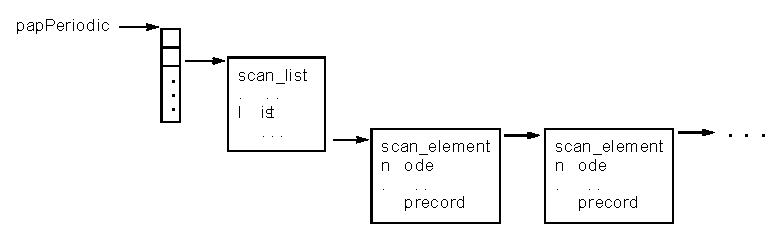
\includegraphics{scanning_19}
\end{center}

When \verb|scanAdd| or \verb|scanDelete| are called, they call the device support routine \verb|get_ioint_info| which returns \verb|pioscanpvt|.
The \verb|scan_element| is added or deleted from the correct scan list.

\subsubsection{scanIoRequest}

\begin{verbatim}
scanIoRequest (IOSCANPVT pioscanpvt)
\end{verbatim}

\index{scanIoRequest}This routine is called to request I/O event scanning.
It can be called from interrupt level.
It looks at each \verb|io_scan_list| referenced by \verb|pioscanpvt| (one for each callback priority) and if any elements are present in the \verb|scan_list| a \verb|callbackRequest| is issued.
The appropriate callback task calls routine \verb|ioeventCallback|, which just calls \verb|scanList|. 

\subsection{Periodic Scanning}

\index{Periodic Scanning}
Periodic scanning is built around the following definitions:

\begin{verbatim}
typedef struct periodic_scan_list {
    scan_list           scan_list;
    double              period;
    volatile enum ctl   scanCtl;
    epicsEventId        loopEvent;
} periodic_scan_list;
static int nPeriodic;
static periodic_scan_list **papPeriodic;
static epicsThreadId *periodicTaskId;
\end{verbatim}

\verb|nPeriodic|, which is determined at \verb|iocInit| time, is the number of periodic rates.
\verb|papPeriodic| is a pointer to an array of pointers to \verb|scan_lists|.
There is an array element for each scan rate.
Thus the structure illustrated in the figure below exists after \verb|iocInit|.

\begin{center}
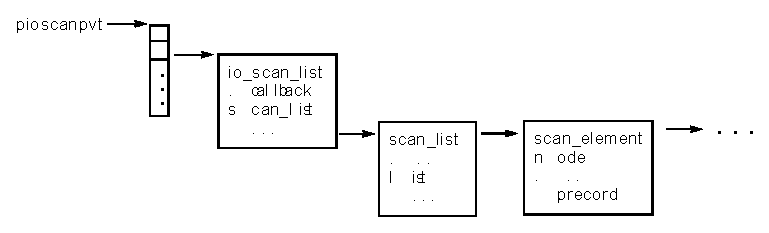
\includegraphics{scanning_1}
\end{center}

A periodic scan task is created for each scan rate.
The following routines implement periodic scanning:

\subsubsection{initPeriodic}

\begin{verbatim}
initPeriodic()
\end{verbatim}

\index{initPeriodic}This routine first determines the scan rates.
It does this by accessing the \verb|SCAN| field of the first record it finds.
It issues a call to \verb|dbGetField| with a \verb|DBR_ENUM| request.
This returns the menu choices for \verb|SCAN|.
From this the periodic rates are determined.
The array of pointers referenced by \verb|papPeriodic| is allocated.
For each scan rate a \verb|scan_list| is allocated and a \verb|periodicTask| is spawned.

\subsubsection{periodicTask}

\begin{verbatim}
periodicTask (struct scan_list *psl)
\end{verbatim}

\index{periodicTask}This task just performs an infinite loop, calling \verb|scanList| and then waiting until the start of the next scan interval, allowing for the time it took to scan the list.
If a periodic scan list takes longer to process than its defined scan period, the next scan will be delayed by half a scan period, with a maximum of 1 second delay.
This does not limit what scan rates can actually be implemented, as long as all the records in the list can be processed within the requested period.
Persistent over-runs (more than 10 times in a row) will result in a warning message being logged.
The total number of over-runs is counted by each scan thread and can be displayed using the \verb|scanppl| command.

\subsection{Scan Once}

\subsubsection{scanOnce}

\begin{verbatim}
void scanOnce (dbCommon *precord)
\end{verbatim}

\index{scanOnce}A task \verb|onceTask| waits for requests to issue a \verb|dbProcess| request.
The routine \verb|scanOnce| puts the address of the record to be processed in a ring buffer and wakes up \verb|onceTask|.

This routine can be called from interrupt level.

\subsubsection{SetQueueSize}

\verb|scanOnce| places its request on a ring buffer.
This is set by default to 1000 entries.
It can be changed by executing the following command in the startup script before \verb|iocInit|:

\begin{verbatim}
int scanOnceSetQueueSize(int size);
\end{verbatim}

\index{scanOnceSetQueueSize}

